\documentclass[tikz,border=12pt]{standalone}
% Estilo comum dos esquemas vetoriais das aulas da GA033.
\usepackage[T1]{fontenc}
\usepackage[utf8]{inputenc}
\usepackage{lmodern}
\usepackage{amsmath,amssymb}
\usetikzlibrary{arrows.meta,positioning,calc,fit,matrix,decorations.pathreplacing,backgrounds,shapes.geometric}
\definecolor{lnccblue}{HTML}{075AC0}
\definecolor{ink}{HTML}{242A31}
\definecolor{muted}{HTML}{647080}
\definecolor{lightblue}{HTML}{EFF5FC}
\definecolor{teal}{HTML}{197C83}
\definecolor{orange}{HTML}{BC6A16}
\tikzset{
  every node/.style={font=\sffamily\fontsize{15}{18}\selectfont,text=ink},
  box/.style={draw=lnccblue,line width=0.9pt,fill=lightblue,inner sep=9pt,align=center},
  flow/.style={-{Stealth[length=3mm,width=2mm]},draw=lnccblue,line width=1pt},
  point/.style={circle,draw=lnccblue,fill=white,line width=1.2pt,minimum size=3.2mm,inner sep=0pt},
  label/.style={font=\sffamily\fontsize{13}{16}\selectfont,text=muted},
  heading/.style={font=\sffamily\bfseries\fontsize{16}{19}\selectfont,text=lnccblue}
}
% Impede setas horizontais involuntariamente invertidas após editar os nós.
\newdimen\origemseta
\newdimen\destinoseta
\newcommand{\verificarsetadireita}[2]{%
  \pgfextractx{\origemseta}{\pgfpointanchor{#1}{east}}%
  \pgfextractx{\destinoseta}{\pgfpointanchor{#2}{west}}%
  \advance\origemseta by 4mm%
  \ifdim\destinoseta>\origemseta\else
    \PackageError{diagramas}{Conector sem espaco entre #1 e #2}{Afaste os nos antes de compilar.}%
  \fi
}

\begin{document}
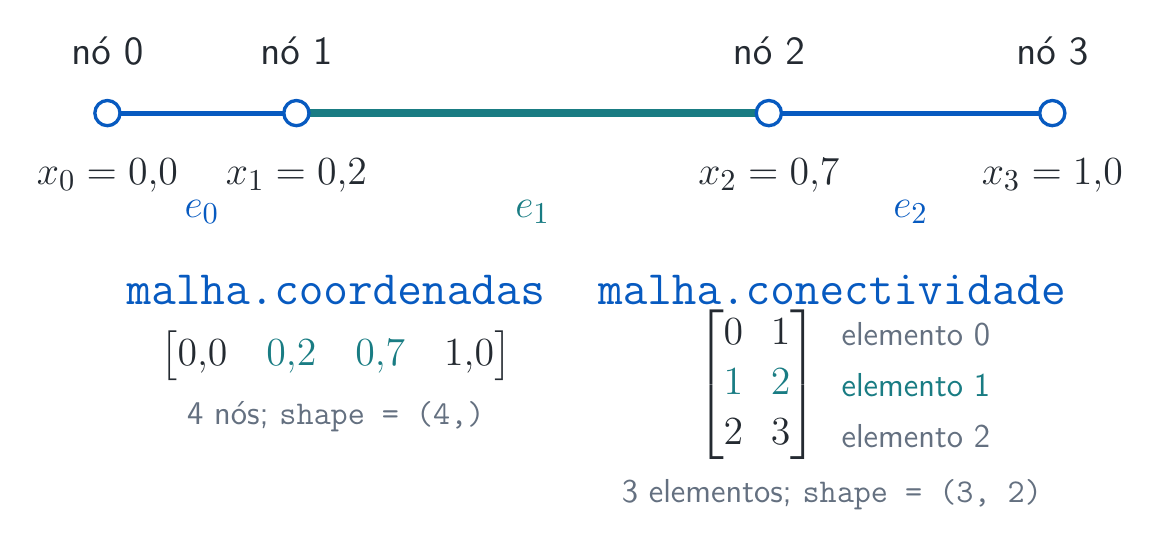
\begin{tikzpicture}
  \coordinate (n0) at (0.5,3.4);
  \coordinate (n1) at (2.9,3.4);
  \coordinate (n2) at (8.9,3.4);
  \coordinate (n3) at (12.5,3.4);
  \draw[lnccblue,line width=1.8pt] (n0) -- (n1);
  \draw[teal,line width=2.8pt] (n1) -- (n2);
  \draw[lnccblue,line width=1.8pt] (n2) -- (n3);
  \foreach \i/\valor in {0/0{,}0,1/0{,}2,2/0{,}7,3/1{,}0} {
    \node[point] at (n\i) {};
    \node[above=14pt] at (n\i) {nó \i};
    \node[below=13pt] at (n\i) {$x_{\i}=\valor$};
  }
  \node[text=lnccblue] at (1.7,2.15) {$e_0$};
  \node[text=teal] at (5.9,2.15) {$e_1$};
  \node[text=lnccblue] at (10.7,2.15) {$e_2$};
  \node[heading] at (3.4,1.15) {\texttt{malha.coordenadas}};
  \node at (3.4,0.32) {$\bigl[0{,}0\quad\color{teal}0{,}2\quad\color{teal}0{,}7\quad\color{ink}1{,}0\bigr]$};
  \node[label] at (3.4,-0.45) {4 nós; \texttt{shape = (4,)}};
  \node[heading] at (9.7,1.15) {\texttt{malha.conectividade}};
  \node at (8.75,-0.05) {$\begin{bmatrix}0 & 1\\\color{teal}1 & \color{teal}2\\2 & 3\end{bmatrix}$};
  \node[label,anchor=west] at (9.7,0.60) {elemento 0};
  \node[label,anchor=west,text=teal] at (9.7,-0.05) {elemento 1};
  \node[label,anchor=west] at (9.7,-0.70) {elemento 2};
  \node[label] at (9.7,-1.45) {3 elementos; \texttt{shape = (3, 2)}};
\end{tikzpicture}
\end{document}
